\section{Aufgabe 2: Evaluierung von Caching Methoden einer Browser Extension}
\label{s:evaluierungcaching}


\subsection{Speichern von Informationen}
\label{ss:speichern}

Bevor diese Arbeit mögliche Methoden zur Speicherung von Datensätzen evaluiert, werden zuerst grundlegende Fragen beantwortet:

\textbf{Warum benötigt die Extension einen Cache?}:
In Kapitel \ref{ss:aufbauwebsite} zeigt die Abbildung \ref{playstore1} den Aufbau der Internetseite nach bestimmten Themen. Jedes Thema wird mit einer Reihe von Apps dargestellt. Je nach Bildschirmauflösung beinhaltet eine Reihe 7 bis 10 dieser Kacheln.
Beim initialen Aufruf lädt die Seite 8 Themen. Weitere Reihen werden dynamisch beim Scrollen nachgeladen. So findet die Extension zwischen 60 bis 80 App-IDs allein durch den Aufruf der Seite. Wird eine Thema durch den Button \glqq Mehr\grqq{} aufgeklappt, lädt die Seite 120 bis 540 weitere Kacheln. Dabei sind Applikationen oft in mehr als einem Thema vorhanden und bereits auf der Startseite doppelt oder dreifach abgebildet.

Da die Extension pro gefundener App-ID eine Anfrage an das Backend schickt. Entstehen pro Seitenaufruf mindestens 60 und pro Klick auf ein Themengebiet mindestens weitere 120 Anfragen. Also würde ein Nutzer bei einem Besuch der Seite grob geschätzt mehrere hunderte Backend-Anfragen auslösen.

Da diese Webseite als Such- und Einkaufsplattform fungiert, bleibt es in der Regel nicht bei einem einzigen Besuch. Hinzu kommt also eine hohe Redundanz der Anfragen bei erneutem Besuch der Seite. Denn viele Themen und Kategorien, wie zum Beispiel \glqq Empfehlungen für dich \grqq{} sind personalisiert und bleiben über eine Vielzahl an Seitenaufrufen identisch.

Zusammenfassend entstehen bei der Nutzung des Google Play Stores also eine hohe Anzahl an benötigten Informationen mit einer Vielzahl an Redundanz sowohl bei einem Besuch, als auch über mehrere Sitzungen hinweg. Die Veröffentlichung der Extension würde also einen hohes Anfrageaufkommen an das Backend verursachen. Durch eine folgende Überlastung könnte die Extension keine Informationen mehr darstellen und hätte keinen Nutzen mehr.

Der Lösungsansatz ist ein, vom Backend unabhängiger, Speicher, welcher gewonnene Informationen für den Nutzer bereithält. Vor allem langlebige und redundante Daten stehen so ohne wiederholte Anfragen zur Verfügung.


\textbf{Welche Informationen sollen im Cache gespeichert werden?}:
Damit nicht nur die Anzahl der Anfragen an das Backend, sondern auch der Umfang der Daten möglichst gering bleibt, werden die nötigten Informationen und ihrer komprimierten Form angefragt. Dem Backend wird durch bestimmte Parameter signalisiert, nur die Kennzahl der zutreffenden Infobox(siehe Tabellen \ref{tabelleInfofelder} und  \ref{tabelleInfofelderzwei}) zusammen mit der Extraktionsquelle und dem Datum der Extraktion zu der jeweiligen App-ID zu übermitteln.

So entsteht folgender key-value-Datensatz:

\big\{ \textbf{key}: \textit{App-ID}, \textbf{value}: \textit{Extraktionstag in Tagen},\textit{Array von Infoboxen als Zahlen} \big\}

\begin{figure}[ht]
	\centering
	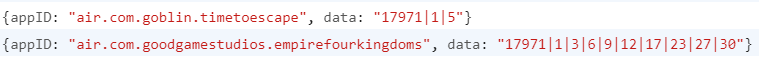
\includegraphics[width=1\textwidth]{pics/cache1.png}
	\caption{Beispiel eines key-value-Datensatzes}
	\label{cache1}
\end{figure}


Die gespeicherten Indizes der Infoboxen werden lokal von der Extension über die Datei \glqq IB\_texte.json \grqq{}(Auszug in Abbildung \ref{cache2}) auf ihre entsprechenden Texte gemappt, sodass diese nicht über das Backend abgefragt werden müssen. Der Extraktionstag dient zur Feststellung des Alters eines Datensatzes. Aktuell ist festgelegt, dass eine Information dann als veraltet gilt, wenn ihr Extraktionsdatum älter als drei Tage ist. Erst sobald die Zeitspanne überschritten wurde, sendet die Extension mit dem nächsten Aufruf der jeweiligen Applikation eine neue Anfrage.


\lstinputlisting[label={cache2},caption={Infobox 19 aus der IB\_texte.json}, firstline=442, lastline=470]{../../Extension/src/lib/data/IB_texte.json}

\textbf{Wie viele Informationen können gespeichert werden?}:
Für die oben gezeigte Struktur der Datensätze ergibt sich folgender \textit{worst-case}:

\textbf{key}: \big\{ \textit{max. 50 characters}\footnote{Gemessen durch Analyse aller App-ID-Einträge während der Evaluation} \big\}

\textbf{value}: \big\{\textit{99999,1,2,3,4,5,6,7,8,9,10,11,12,13,14,15,16,17,}
	
\textit{18,19,20,21,22,23,24,25,26,27,28,29,30,31} \big\}

Das entspricht einer Länge von 50 characters für den key und 89 characters für den value. In UTF-8 sind das umgerechnet ca. 139Byte. Geht man in Google Chrome von einem Limit des Cache-Speichers auf 5200000 characters\footnote{\url{https://arty.name/localstorage.html}} aus, können so ca. 37410 Datensätze gespeichert werden.

\subsection{Kriterien und Vorauswahl}
\label{vorauswahl}


Welche Arten von Speicher stehen einer Extension für Browser (hier Chrome) zur Verfügung?

Integriert: Session Storage und lokal Storage
Session Storage: Daten bleiben nur während der Sitzung erhalten. Das Schließen des Browsers bzw. das Öffnen der Website in einem anderen Tab/Browserfenster beendet die Sitzung

Local Storage: Daten bleiben über eine Sitzung hinaus erhalten und verfallen erst durch Überschreiben oder Löschen

Kapazität: 5MB

Aufbau: String-Tupel nach dem (Key, Value)-Prinzip

Zugriff: getItem(key), setItem(key,value) und removeItem(key)


Serverseitiger Speicher:
Identifizierung notwendig. Aufwendig in Pflege und Wartung. Kein Mehrwert zu Anfragen an Informationsquelle

Serverseitiger Speicher fällt vor vorne herein weg aus oben genannten Grund und datenschutzrechtlichen Bedenken.


Datenbanken:
Verfügbar: IndexedDB und WebSQL

WebSQL seit November 2010 von W3C nicht mehr empfohlen (veraltet).

IndexedDB: API in allen modernen Browser zur Speicherung von Daten und Dateien in einer object-orientierten Datenbank.
synchron und asynchron möglich.
Funktioniert nach key, value prinzip
Alle Datentypen von JavaScript werden unterstützt.
Kann indexiert werden um Suchen effizient zu machen.
Verwendet Prinzip von Transaktionen
Anfragen mit Rückgabewerten als Basis aller Operationen
Verfolgt den NoSQL-Ansatz


Speicherlimit nach global Limit (1/2 Festplatte) und Gruppenlimit (1/5 von global Limit, min 10MB max. 2GB)
Gruppenlimit voll = voll (Fehler)
Global Limit voll = löschen bis wieder frei (Quellenabhängig komplette Elemente gelöscht)

Warum nicht IndexedDB?

Vorteile von IndexedDB: Abspeicherung von großen strukturierten Datenmengen.
Nachteile: hoher Aufwand bei Implementierung.Overhead lohnt nicht bei kleinen Datenmengen. Transaktionen blockieren bei Fehlern  eventuell den Datenabruf bzw. die Aktualisierung

Storage API von Chrome ausreichend Speicher und geringer aufwand bei der Implementierung. Lediglich Strings benötigt. Indices bei gewählen value-Struktur nicht notwendig.

Vorteil von Session Storage: Speicherpflege nicht notwendig, da 5MB groß genug für Anzahl(?) an App-Informationen während einer Session im PlayStore. Informationen immer auf Stand der Quelle
Nachteil: Bei erstmaligen Öffnen des Stores in neuer Browsersession werden viele Anfragen losgeschickt für Apps die bereits in der letzten Session schon angefragt wurden. Bei Serverausfällen fehlen die Informationen
Lediglich in einer Session mehrfach aufgerufene Apps ersparen erneute Anfragen.
=> Speicherpflege fällt weg, dafür kaum Mehrwert bei Anfragen.

Vorteil von Lokal Storage: Apps werden einmal abgefragt und sind anschließend abgespeichert. Fällt der Server aus können die lokalen Informationen genutzt werden. Daten auch aus letzter Session bleiben vorhanden. Neue Anfragen werden nur dann geschickt wenn aktuelle Daten über 3 Tage alt sind.
Nachteile: Speicherpflege notwendig. Dadurch wird die Information länger (Counter und Tag). Zusätzliche Rechenzeit für das Löschen von alten Informationen notwendig. Dadurch wird sichergestellt dass die 5MB nicht überschritten werden und somit Informationen ungewollt verloren gehen. Für Informationen mit hohem Counter muss regelmäßig überprüft werden, ob die Information noch aktuell ist, weil diese in der Regel lange im Speicher verweilt.
=> Hohe Einsparung bei Anfragen an den Server möglich. Dafür müssen zusätzliche Operationen zur Speicherpflege und Prüfung der Informationen ausgeführt werden.

\subsection{Vorgehensweise}
\label{ss:vorgehensweise}

Plattform: Windows 10 Rechner Build, Specs
Chrome Details
App Details
Was wird gemessen?
Limitierungen

Getestet auf:

Windows 10 Education 64 Bit
Build 10.0.17134
Prozessor i7-6700K
RAM: 16GB
GPU: Nvidia GTX 1070

Chrome  67.0.3396.99 64 Bit

\subsection{Ergebnisse}
\label{ss:ergebnisseht2}

Storage: none
Ladezeit: 1435ms
Start der Extension-Funktionsaufrufe: 944ms
Dauer: 491ms
Anzahl der Anfragen an das Backend: 0


Storage: Local Storage
Ladezeit: 1711ms
Start der Extension-Funktionsaufrufe: 892ms
Dauer: 819ms
Anzahl der Anfragen an das Backend: 125


Storage: none
Ladezeit: 1761ms
Start der Extension-Funktionsaufrufe: 883ms
Dauer: 878ms
Anzahl der Anfragen an das Backend: 131




\subsection{Diskussion}
\label{ss:diskussionht2}

Zeitspanne verlängern